\section{Monitoring et Backups}

\subsection{Monitoring}
Afin d'être tenu au courant de l'état de l'application web, il st important de mettre en place un système de monitoring. OVH met à disposition un panneau de contrôle permettant de visualiser certaines informations propre au VPS tel que l'utilisation du CPU, de la mémoire ou encore le traffic réseau. Ces informations sont intéressantes dans le but de déterminer si les performances du VPS conviennent pour l'application mais ne permettent pas de déceler une éventuelle indisponibilité de l'application. 

\newpara

Dès lors, dans le but de connaître l'état de disponibilité de l'application, j'ai utilisé "UptimeRobot"\footnote{\url{https://uptimerobot.com}}. En plus de pouvoir consulter l'état de disponibilité sur l'application web, celle-ci peut envoyer un email d'alerte dans l'éventualité ou le site serait indisponible.

\begin{figure}[H]
  \centering
  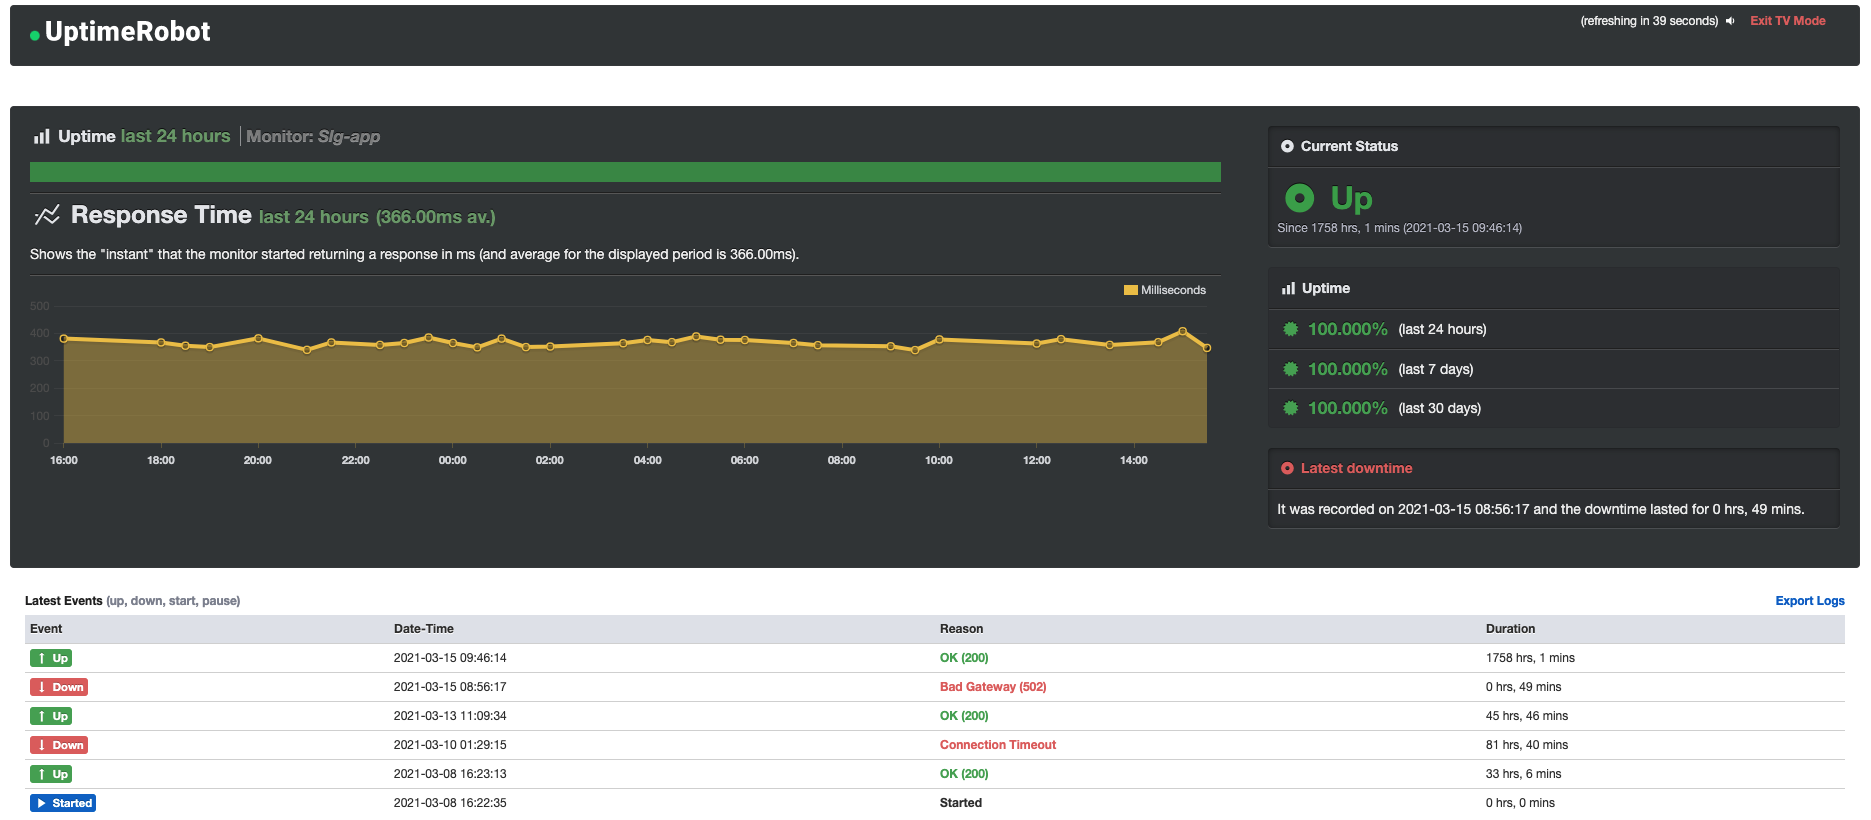
\includegraphics[width=\linewidth]{img/uptimeRobot.png}
  \caption{Dashboard monitoring de l'application - UptimeRobot}
\end{figure}

\newpara

Dans le future il serait intéressant de mettre en place un monitoring plus approfondi permettant de récupérer des informations plus détaillée à partir des conteneurs docker. Ceci peut être obtenu à l'aie d'outils tel que "Prometheus"\footnote{\url{https://prometheus.io}} ou "Sematext"\footnote{\url{https://sematext.com/docker/}} 

\newpage

\subsection{Backups}

Comme expliqué dans la seconde partie du \textit{chapitre \ref{scritps}}, actuellement un backup de la base de données est effectué quotidiennement. Cependant ces backups sont stockés sur le VPS lui-même. En cas de perte du VPS, les backups sont eux aussi perdus.

\newpara

A terme, il faudra externaliser les backups. OVH propose une solution payante à laquelle nous souscrirons probablement une fois l'application terminée dans son intégralité.